%To compile as handout, use
%pdflatex "\def\ishandout{1} \input{filename.tex}"
%Defaults to non-handout mode (with slide reveals)
\ifdefined\ishandout
  \documentclass[handout]{beamer}
\else
  \documentclass{beamer}
\fi
 
\usepackage{econ103slides} 

\date{Lecture \# 7}
\begin{document} 

%%%%%%%%%%%%%%%%%%%%%%%%%%%%%%%%%%%%%%%%

\begin{frame}[plain]
	\titlepage 
	

\end{frame} 

%%%%%%%%%%%%%%%%%%%%%%%%%%%%%%%%%%%%%%%%
\begin{frame}
\begin{center}
 \Huge Basic Probability -- Part III
\end{center}

\end{frame}


%%%%%%%%%%%%%%%%%%%%%%%%%%%%%%%%%%%%%%%%
%Some macros for the Venn Diagrams
\def\EventA{(-0.35,0) circle (1.2)}
\def\EventB{(1.35,0) circle (1.2)}
\def\EventC{(-0.35,0) circle (0.6)}
\def\EventD{(0,0) circle (1.6)}
\def\SampleSpace{(-2,-2) rectangle (3,2)}
%%%%%%%%%%%%%%%%%%%%%%%%%%%%%%%%%%%%%%%%

%\begin{frame}
%\frametitle{Recall from Last Time: Conditional Probability}
%\framesubtitle{Set of relevant outcomes restricted by condition}
%$$P(A|B) = \frac{P(A\cap B)}{P(B)},\;\; \mbox{provided } P(B)>0$$
%\begin{figure}
%\centering
%\begin{tikzpicture}[scale = 1]
%
%	\begin{scope}[fill opacity = 0.5]
%		\fill[red] \EventB;
%      	\clip \EventA;
%      	\fill[blue] \EventB;
%    \end{scope}
%	\draw \EventA node [above] {$A$};
%	\draw \EventB node [above] {$B$};
%      \draw \SampleSpace node [right] {$S$};
%\end{tikzpicture}
%\caption{$B$ becomes the ``new sample space'' so we need to re-scale by $P(B)$ to keep probabilities between zero and one.}
%\end{figure}
%\end{frame}
%%%%%%%%%%%%%%%%%%%%%%%%%%%%%%%%%%%%%%%%%
%
%\begin{frame}
%\frametitle{Independence and The Multiplication Rule}
%\begin{block}{The Multiplication Rule}
%Just rearrange the definition of conditional probability:
%$P(A\cap B) = P(A|B)P(B)$
%\end{block}\pause
%\begin{block}{Statistical Independence}
%$P(A\cap B) = P(A)P(B)$
%\end{block}\pause
%\begin{alertblock}{By the Multiplication Rule}
%$\mbox{Independence } \iff P(A|B) = P(A)$\\
%\end{alertblock}\pause
%\begin{block}{Interpreting Independence}
%Knowing that $B$ has occurred doesn't give us any additional information about whether $A$ will.
%\end{block}
%\end{frame}
%%%%%%%%%%%%%%%%%%%%%%%%%%%%%%%%%%%%%%%%%
%
%\begin{frame}
%\frametitle{Will Having 5 Children Guarantee a Boy? \hfill 
\includegraphics[scale = 0.05]{./images/clicker}}
%A couple plans to have five children. Assuming that each birth is independent and male and female children are equally likely, what is the probability that they have at least one boy?
%\vspace{1em}
%
%\pause
%\alert{By Independence and the Complement Rule,}
%	\begin{eqnarray*}
%		P(\mbox{no boys})&=&\pause P(\mbox{5 girls})\\
%							&=&\pause 1/2 \times 1/2 \times 1/2 \times 1/2 \times 1/2\\
%							&=&\pause 1/32\\ \\ \pause
%		P(\mbox{at least 1 boy})&=&\pause1 - P(\mbox{no boys})\\
%		&=&\pause1 - 1/32 =\pause 31/32 = 0.97
%	\end{eqnarray*}
%
%\end{frame}
%%%%%%%%%%%%%%%%%%%%%%%%%%%%%%%%%%%%%%%%%
%
%
%\begin{frame}
%\frametitle{The Law of Total Probability}
%If $E_1, E_2, \hdots, E_k$ are mutually exclusive, collectively exhaustive events and $A$ is another event, then
%	$$P(A) = P(A|E_1)P(E_1) + P(A|E_2)P(E_2) + \hdots + P(A|E_k)P(E_k)$$
%
%\end{frame}
%%%%%%%%%%%%%%%%%%%%%%%%%%%%%%%%%%%%%%%%%
%%Some macros for the Venn Diagrams
%\def\EventA{(-0.35,0) circle (1.2)}
%\def\EventB{(1.35,0) circle (1.2)}
%\def\EventC{(-0.35,0) circle (0.6)}
%\def\EventD{(0,0) circle (1.6)}
%\def\SampleSpace{(-2,-2) rectangle (3,2)}
%%%%%%%%%%%%%%%%%%%%%%%%%%%%%%%%%%%%%%%%%
%\begin{frame}
%\frametitle{Deriving the Law of Total Probability For $k=2$}
%
%\begin{columns}
%
%\column{0.7\textwidth}
%\uncover<2->{
%
%Since $A\cap B$ and $A \cap B^c$ are mutually exclusive and their union equals $A$,
%	$$P(A) = P(A\cap B) + P(A \cap B^c)$$}
%	\uncover<3->{
%But by the multiplication rule:
%	\begin{eqnarray*}
%		P(A\cap B)&=&P(A|B)P(B)\\
%		P(A \cap B^c)&=&P(A|B^c)P(B^c)
%	\end{eqnarray*}}
%\uncover<4->{
%Combining,
%	$$\alert{P(A) = P(A|B)P(B) + P(A|B^c)P(B^c)}$$}
%\column{0.3\textwidth}
%\uncover<1->{
%\begin{figure}
%\centering
%\begin{tikzpicture}[scale = 0.5]
%
%	\begin{scope}[fill opacity = 0.5]
%		\fill[red] \EventB;
%      	\clip \EventA;
%      	\fill[blue] \EventB;
%    \end{scope}
%	\draw \EventA node [above] {$B$};
%	\draw \EventB node [above] {$A$};
%      \draw \SampleSpace node [right] {$S$};
%\end{tikzpicture}
%\caption{$A = (A\cap B) \cup (A \cap B^c)$, $(A\cap B) \cap (A \cap B^c) = \emptyset$}
%\end{figure}}
%
%\end{columns}
%
%\end{frame}
%%%%%%%%%%%%%%%%%%%%%%%%%%%%%%%%%%%%%%%%%
%
%\begin{frame}
%\frametitle{Connecticut, 2006 -- Democratic Primary for Senate Race}
%
%
%\begin{figure}
%	\fbox{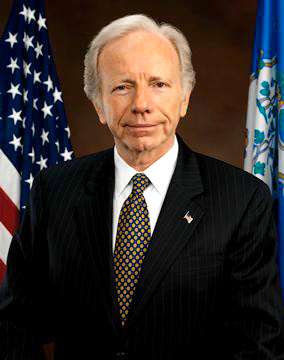
\includegraphics[scale = 0.26]{./images/lieberman}}
%	\hspace{1em}
%	\fbox{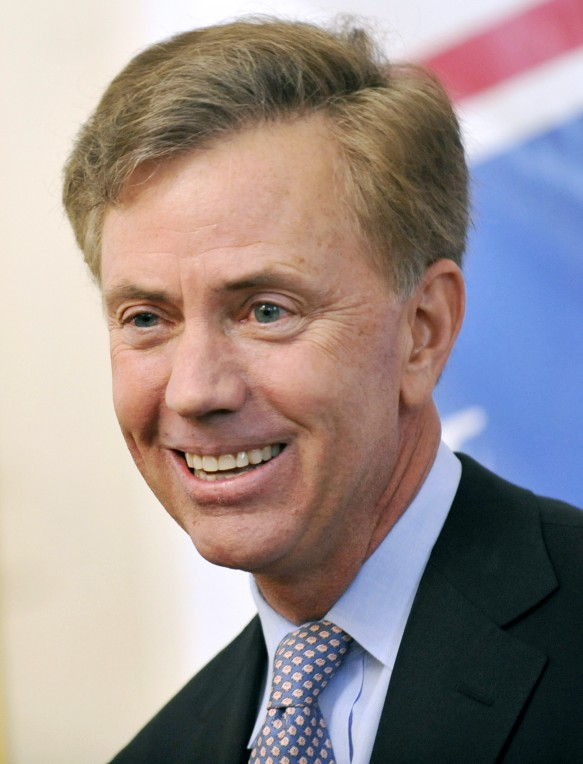
\includegraphics[scale = 0.123]{./images/lamont}}
%	\caption{Former Senator Joe Lieberman and never-Senator  Ned Lamont. In 2006 Lieberman, a popular Democratic incumbant, faced a primary challenge from Lamont, because of the former's support for George W.\ Bush's foreign policy agenda.}
%\end{figure}
%
%\end{frame}
%%%%%%%%%%%%%%%%%%%%%%%%%%%%%%%%%%%%%%%%%
%\begin{frame}
%
%\frametitle{How do prediction markets work?}
%\framesubtitle{To learn more, see \fbox{\href{http://www.aeaweb.org/articles.php?doi=10.1257/0895330041371321}{Wolfers \& Zitzewitz (2004)}}}
%\begin{center}
%\fbox{\fbox{\begin{minipage}{0.5\textwidth}
%\textsc{This certificate entitles the bearer to \$10 if Duke wins the Final Four in 2016.}
%\end{minipage}}}
%\vspace{1em}
%\pause
%\begin{block}{Buyers -- Purchase Right to Collect}\pause
%Duke very likely to win $\Rightarrow$ buy for close to \$10. \pause \\Duke very unlikely to win $\Rightarrow$ buy for close to \$0. \pause
%\end{block}
%
%\begin{block}{Sellers -- Sell Obligation to Pay} \pause
%Duke very likely to win $\Rightarrow$ sell for close to \$10. \pause \\Duke very unlikely to win $\Rightarrow$ sell for close to \$0.
%\end{block}
%\end{center}
%
%\end{frame}
%%%%%%%%%%%%%%%%%%%%%%%%%%%%%%%%%%%%%%%%%
%\begin{frame}
%
%\Large Going price of contract encodes market participants' beliefs in the form of probability:
%\Large\\ 
%$$\mbox{Price}/\$10 \approx \mbox{Subjective Probability}$$
%
%
%\end{frame}
%%%%%%%%%%%%%%%%%%%%%%%%%%%%%%%%%%%%%%%%%
%\begin{frame}
%\frametitle{Summer 2006 -- Two Contracts on Tradesports}
%\uncover<1>{\alert{What is the missing probability? \hfill  
\includegraphics[scale = 0.05]{./images/clicker} }}
%
%\begin{table}
%\begin{tabular}{l|ll}
%	Contract -- Pays \$10 if Event Occurs & Price & Prob.\ \\
%	\hline
%	Lieberman Wins CT Dem.\ Senate Primary& \$3.20&\uncover<2->{\alert{0.32}}\\
%	Neither Dem.\ nor Rep.\ wins CT Senate Election&\$3.01&0.3
%\end{tabular}
%\end{table}
%
%\vspace{1em}
%\begin{alertblock}{But the real question of interest was whether Lieberman would keep his Senate seat. Can we calculate the implied probability?}\end{alertblock}
%\end{frame}
%%%%%%%%%%%%%%%%%%%%%%%%%%%%%%%%%%%%%%%%%
%\begin{frame}
%%\frametitle{Perhaps we can \emph{calculate} the missing probability...}
%\fbox{\begin{minipage}{0.9\textwidth}
%\footnotesize
%$K$ = Joe Lieberman keeps his Senate seat \\ 
%$N$ = Neither Dem.\ nor Rep.\ wins Senate seat  (Tradesports Prob.\ 0.3)\\
%$J =$ Joe Lieberman wins the Dem.\ Primary (Tradesports Prob.\ 0.32)
%\end{minipage}}
%\normalsize
%\vspace{1em}
%
%\begin{block}{Law of Total Probability }
%\begin{eqnarray*}
%	P(K) &=& \pause P(K|J)P(J) + P(K|J^c)P(J^c)\\
%		&=&\pause P(K|J)  \times \alert{0.32} + P(K|J^c) \times \alert{(1 - 0.32)} \pause
%\end{eqnarray*}
%\end{block}
%\begin{block}{No serious Republican Challengers $\Rightarrow P(K|J) \approx 1$}\pause
%	$$P(K) \approx 0.32 + \alert{P(K|J^c)} \times 0.68$$
%\end{block}
%\end{frame}
%%%%%%%%%%%%%%%%%%%%%%%%%%%%%%%%%%%%%%%%%
%\begin{frame}
%%\frametitle{But what is $P(K|J^c)$?}
%\fbox{\begin{minipage}{0.9\textwidth}
%\footnotesize
%$K$ = Joe Lieberman keeps his Senate seat \\ 
%$N$ = Neither Dem.\ nor Rep.\ wins Senate seat  (Tradesports Prob.\ 0.3)\\
%$J =$ Joe Lieberman wins the Dem.\ Primary (Tradesports Prob.\ 0.32)
%\end{minipage}}
%\normalsize
%\vspace{1em}
%
%\begin{block}{Law of Total Probability Again}
%	\begin{eqnarray*}
%	P(N) &=& \pause P(N|J)P(J) + P(N|J^c)P(J^c)\\ \pause
%	\alert{0.3} &=& P(N|J)\times \alert{0.32} + P(N|J^c)\times \alert{0.68}\\
%	\end{eqnarray*}
%\end{block}\pause
%\begin{block}{No serious Independent challengers $\Rightarrow P(N|J) \approx 0$}
%\begin{eqnarray*}\pause
%	\alert{0.3} &\approx&  P(N|J^c)\times \alert{0.68}\\ \pause
%	P(N|J^c) &\approx& 0.44
%	\end{eqnarray*}
%\end{block}
%\end{frame}
%%%%%%%%%%%%%%%%%%%%%%%%%%%%%%%%%%%%%%%%%
%\begin{frame}
%%\frametitle{But I thought we wanted $P(K|L^c)$!}
%\fbox{\begin{minipage}{0.9\textwidth}
%\footnotesize
%$K$ = Joe Lieberman keeps his Senate seat \\ 
%$N$ = Neither Dem.\ nor Rep.\ wins Senate seat  (Tradesports Prob.\ 0.3)\\
%$J =$ Joe Lieberman wins the Dem.\ Primary (Tradesports Prob.\ 0.32)
%\end{minipage}}
%\normalsize
%\vspace{1em}
%\begin{alertblock}{Since Lieberman will run as an Independent if he loses the primary and there are no serious Independent challengers:}
%	$$P(K|J^c) \approx P(N|J^c) \approx 0.44$$
%\end{alertblock}
%\end{frame}
%%%%%%%%%%%%%%%%%%%%%%%%%%%%%%%%%%%%%%%%%
%
%\begin{frame}
%\frametitle{We \emph{can} calculate the missing probability!}
%\fbox{\begin{minipage}{0.9\textwidth}
%\footnotesize
%$K$ = Joe Lieberman keeps his Senate seat \\ 
%$N$ = Neither Dem.\ nor Rep.\ wins Senate seat  (Tradesports Prob.\ 0.3)\\
%$J =$ Joe Lieberman wins the Dem.\ Primary (Tradesports Prob.\ 0.32)
%\end{minipage}} 
%\normalsize
%\vspace{2em}
%\begin{alertblock}{Combining the Tradesports prices with the assumptions of no serious Republican or Independent Challengers:}
%	\begin{eqnarray*}
%		P(K)&=&  P(K|J)P(J) + P(K|J^c)P(J^c)\\
%		\pause &\approx& 0.32 + \alert{P(K|J^c)} \times 0.68\\
%		\pause &\approx& 0.32 + \alert{0.44} \times 0.68\\
%		\pause &\approx& \alert{0.62} 
%	\end{eqnarray*}
%\end{alertblock}
%\end{frame}
%%%%%%%%%%%%%%%%%%%%%%%%%%%%%%%%%%%%%%%%%
%\begin{frame}
%\frametitle{Wait, isn't that just 0.3 + 0.32?}
%\fbox{\begin{minipage}{0.9\textwidth}
%\footnotesize
%$K$ = Joe Lieberman keeps his Senate seat \\ 
%$N$ = Neither Dem.\ nor Rep.\ wins Senate seat  (Tradesports Prob.\ 0.3)\\
%$J =$ Joe Lieberman wins the Dem.\ Primary (Tradesports Prob.\ 0.32)
%\end{minipage}} 
%\normalsize
%\vspace{2em}
%
%You may have noticed that the answer we ended up with was 0.62, which is \emph{identical} to simply adding up the Tradesports probabilities of $N$ and $J$. 
%
%
%\vspace{1em}
%\alert{Essentially, the assumptions we made are equivalent to assuming that $K = N \cup J$ \emph{and} that $N$ and $J$ are mutually exclusive events. Since the probabilities of mutually exclusive events sum: $P(K) = P(N\cup J) = P(N) + P(J)$. }
%
%\end{frame}
%%%%%%%%%%%%%%%%%%%%%%%%%%%%%%%%%%%%%%%%%
%\begin{frame}
%\frametitle{What Actually Happened?}
%
%Ned Lamont won the Democratic Primary with 52\% of the vote, but Joe Liberman ran as an independent in the General Election and won. Lieberman retired from the Senate in January 2013.
%
%\end{frame}
%%%%%%%%%%%%%%%%%%%%%%%%%%%%%%%%%%%%%%%%%
%\begin{frame}
%\frametitle{Why are calculations like this interesting?}
%	\begin{alertblock}{Statistical Arbitrage}
%	If the probabilities implied by the prices of prediction market contracts violate any of the rules we have studied in this class, there is a \emph{pure arbitrage opportunity}, i.e.\ a way make to make a guaranteed, risk-free profit.
%	\end{alertblock}
%\end{frame}
%%%%%%%%%%%%%%%%%%%%%%%%%%%%%%%%%%%%%%%%%
%\begin{frame}
%\frametitle{A Simple Example of Statistical Arbitrage}
%\framesubtitle{Courtesy of  \fbox{\href{http://offsettingbehaviour.blogspot.co.nz/2012/11/barriers-to-arbitrage.html}{Eric Crampton}}}
%
%\begin{block}{November 5th, 2012}
%	\begin{itemize}
%		\item\$2.30 for contract paying \$10 if Romney wins on \fbox{\href{http://www.betfair.com/}{BetFair}} 
%		\item \$6.58 for contract paying \$10 if Obama wins on \fbox{\href{http://http://www.intrade.com/}{InTrade}} 
%	\end{itemize}
%\end{block}
%
%\begin{block}{Implied Probabilities}
%	\begin{itemize}
%	\item BetFair: $P(Romney) \approx 0.23$
%	\item InTrade: $P(Obama) \approx 0.66$
%	\end{itemize}
%\end{block}
%
%\begin{alertblock}{What's Wrong with This?}\pause
% Violates complement rule! $P(Obama) = 1 - P(Romney)$ but the implied probabilities here don't sum up to one!
%\end{alertblock}
%
%
%
%\end{frame}
%
%%%%%%%%%%%%%%%%%%%%%%%%%%%%%%%%%%%%%%%%%
%\begin{frame}
%\frametitle{A Simple Example of Statistical Arbitrage}
%\framesubtitle{Courtesy of  \fbox{\href{http://offsettingbehaviour.blogspot.co.nz/2012/11/barriers-to-arbitrage.html}{Eric Crampton}}}
%
%\begin{block}{November 5th, 2012}
%	\begin{itemize}
%		\item\$2.30 for contract paying \$10 if Romney wins on \fbox{\href{http://www.betfair.com/}{BetFair}} 	
%		\item \$6.58 for contract paying \$10 if Obama wins on \fbox{\href{http://http://www.intrade.com/}{InTrade}}
%	\end{itemize}
%\end{block}
%
%\begin{alertblock}{Arbitrage Strategy}\pause
%Buy Equal Numbers of Each \pause
%	\begin{itemize}
%		\item Cost = \$2.30 + \$6.58 =\$8.88 per pair 
%		\item Payout if Romney Wins: \$10 
%		\item Payout if Obama Wins: \$10
%		\item Guaranteed Profit: \$10 - \$8.88 = \$1.12 per pair
%	\end{itemize} 
%
%\end{alertblock}
%
%
%
%\end{frame}
%%%%%%%%%%%%%%%%%%%%%%%%%%%%%%%%%%%%%%%%%
\begin{frame}
\centering \Huge Four Volunteers Please!

\end{frame}
%%%%%%%%%%%%%%%%%%%%%%%%%%%%%%%%%%%%%%%%
\begin{frame}
\frametitle{The Lie Detector Problem}
\begin{block}{From accounting records, we know that 10\% of employees in the store are stealing merchandise.}\end{block}
\begin{block}{The managers want to fire the thieves, but their only tool in distinguishing is a lie detector test that is 80\% accurate:}
	\begin{eqnarray*}
	\mbox{Innocent } &\Rightarrow& \mbox{Pass test with } 80\% \mbox{ Probability}\\
	\mbox{Thief } &\Rightarrow& \mbox{Fail test with } 80\% \mbox{ Probability}
	\end{eqnarray*}
\end{block}

\pause
\begin{alertblock}{What is the probability that someone is a thief \emph{given} that she has failed the lie detector test?\hfill
\includegraphics[scale = 0.03]{./images/clicker} }
\end{alertblock}

\end{frame}
%%%%%%%%%%%%%%%%%%%%%%%%%%%%%%%%%%%%%%%%

\begin{frame}
\frametitle{Monte Carlo Simulation -- Roll a 10-sided Die Twice}
Managers will split up and visit employees. Employees roll the die twice \alert{but keep the results secret!}
\vspace{1em}
\begin{block}{First Roll -- Thief or not?}
$0 \Rightarrow$ Thief, $1-9 \Rightarrow$ Innocent
\end{block}

\begin{block}{Second Roll -- Lie Detector Test}
$0,1 \Rightarrow$ Incorrect Test Result, $2-9$ Correct Test Result
\end{block}
\begin{table}
	\begin{tabular}{l|cc}
	&0 or 1&2--9\\
	\hline
	Thief&Pass&\alert{Fail}\\
	Innocent&\alert{Fail} &Pass
	\end{tabular}
\end{table}

\end{frame}
%%%%%%%%%%%%%%%%%%%%%%%%%%%%%%%%%%%%%%%%
\begin{frame}
\frametitle{What percentage of those who failed the test are guilty?}
\begin{block}{\# Who Failed Lie Detector Test:}

\end{block}


\begin{block}{\# Of Thieves Among Those Who Failed:}

\end{block}

\end{frame}
%%%%%%%%%%%%%%%%%%%%%%%%%%%%%%%%%%%%%%%%
\begin{frame}
\frametitle{Base Rate Fallacy -- Failure to Consider Prior Information}

\begin{block}{Base Rate -- Prior Information}
Before the test we know that 10\% of Employees are stealing.
\end{block}
\vspace{2em}
\begin{alertblock}{People tend to focus on the fact that the test is 80\% accurate and ignore the fact that only 10\% of the employees are theives. }
\end{alertblock}

\end{frame}
%%%%%%%%%%%%%%%%%%%%%%%%%%%%%%%%%%%%%%%%
\begin{frame}
\frametitle{Thief (Y/N), Lie Detector (P/F)}
\footnotesize
\begin{table}
\begin{tabular}{|c|cccccccccc|}
\hline
&0&1&2&3&4&5&6&7&8&9\\
\hline
0&\textcolor{blue}{YP}&\textcolor{blue}{YP}&\textcolor{red}{YF}&\textcolor{red}{YF}&\textcolor{red}{YF}&\textcolor{red}{YF}&\textcolor{red}{YF}&\textcolor{red}{YF}&\textcolor{red}{YF}&\textcolor{red}{YF}\\
1&\textcolor{red}{NF}&\textcolor{red}{NF}&\textcolor{blue}{NP}&\textcolor{blue}{NP}&\textcolor{blue}{NP}&\textcolor{blue}{NP}&\textcolor{blue}{NP}&\textcolor{blue}{NP}&\textcolor{blue}{NP}&\textcolor{blue}{NP}\\
2&\textcolor{red}{NF}&\textcolor{red}{NF}&\textcolor{blue}{NP}&\textcolor{blue}{NP}&\textcolor{blue}{NP}&\textcolor{blue}{NP}&\textcolor{blue}{NP}&\textcolor{blue}{NP}&\textcolor{blue}{NP}&\textcolor{blue}{NP}\\
3&\textcolor{red}{NF}&\textcolor{red}{NF}&\textcolor{blue}{NP}&\textcolor{blue}{NP}&\textcolor{blue}{NP}&\textcolor{blue}{NP}&\textcolor{blue}{NP}&\textcolor{blue}{NP}&\textcolor{blue}{NP}&\textcolor{blue}{NP}\\
4&\textcolor{red}{NF}&\textcolor{red}{NF}&\textcolor{blue}{NP}&\textcolor{blue}{NP}&\textcolor{blue}{NP}&\textcolor{blue}{NP}&\textcolor{blue}{NP}&\textcolor{blue}{NP}&\textcolor{blue}{NP}&\textcolor{blue}{NP}\\
5&\textcolor{red}{NF}&\textcolor{red}{NF}&\textcolor{blue}{NP}&\textcolor{blue}{NP}&\textcolor{blue}{NP}&\textcolor{blue}{NP}&\textcolor{blue}{NP}&\textcolor{blue}{NP}&\textcolor{blue}{NP}&\textcolor{blue}{NP}\\
6&\textcolor{red}{NF}&\textcolor{red}{NF}&\textcolor{blue}{NP}&\textcolor{blue}{NP}&\textcolor{blue}{NP}&\textcolor{blue}{NP}&\textcolor{blue}{NP}&\textcolor{blue}{NP}&\textcolor{blue}{NP}&\textcolor{blue}{NP}\\
7&\textcolor{red}{NF}&\textcolor{red}{NF}&\textcolor{blue}{NP}&\textcolor{blue}{NP}&\textcolor{blue}{NP}&\textcolor{blue}{NP}&\textcolor{blue}{NP}&\textcolor{blue}{NP}&\textcolor{blue}{NP}&\textcolor{blue}{NP}\\
8&\textcolor{red}{NF}&\textcolor{red}{NF}&\textcolor{blue}{NP}&\textcolor{blue}{NP}&\textcolor{blue}{NP}&\textcolor{blue}{NP}&\textcolor{blue}{NP}&\textcolor{blue}{NP}&\textcolor{blue}{NP}&\textcolor{blue}{NP}\\
9&\textcolor{red}{NF}&\textcolor{red}{NF}&\textcolor{blue}{NP}&\textcolor{blue}{NP}&\textcolor{blue}{NP}&\textcolor{blue}{NP}&\textcolor{blue}{NP}&\textcolor{blue}{NP}&\textcolor{blue}{NP}&\textcolor{blue}{NP}\\
\hline
\end{tabular}
\caption{Each outcome in the table is equally likely. The 26 given in red correspond to failing the test, but only 8 of these (YF) correspond to being a thief.}
\end{table}
\end{frame}
%%%%%%%%%%%%%%%%%%%%%%%%%%%%%%%%%%%%%%%%
\begin{frame}
\frametitle{Base Rate of Thievery is 10\%}

% Set the overall layout of the tree
\tikzstyle{level 1}=[level distance=3.5cm, sibling distance=3.5cm]
\tikzstyle{level 2}=[level distance=3.5cm, sibling distance=2.5cm]

% Define styles for bags and leafs
\tikzstyle{bag} = [text width=4em, text centered]
\tikzstyle{end} = [circle, minimum width=3pt,fill, inner sep=0pt]
\tikzstyle{tip} = [circle,fill, minimum height = 3pt, inner sep=0pt]
\begin{figure}
\centering
\begin{tikzpicture}[scale = 0.75,thick,grow=right]
\node[tip]{}
    child {
        node[bag] {Thief}        
        child {
                node[end, label=right:
                    {\alert{\fbox{Fail} $\;\;\; \frac{1}{10} \times \frac{4}{5} = \frac{4}{50}$}}] {}
                edge from parent
                node[below]  {$\frac{4}{5}$}
            }
            child {
                node[end, label=right:
                    {Pass}] {}
                edge from parent
                node[above] {$\frac{1}{5}$}
            }
            edge from parent 
            node[below]  {$\frac{1}{10}$}
    }
    child {
        node[bag] {Honest}        
        child {
                node[end, label=right:
                    {\alert{\fbox{Fail} $\;\;\; \frac{9}{10} \times \frac{1}{5} = \frac{9}{50}$}}] {}
                edge from parent
                node[below]  {$\frac{1}{5}$}
            }
            child {
                node[end, label=right:
                    {Pass}] {}
                edge from parent
                node[above] {$\frac{4}{5}$}
            }
        edge from parent         
            node[above] {$\frac{9}{10}$}
    };
\end{tikzpicture}
\caption{Although $\frac{9}{50} + \frac{4}{50} = \frac{13}{50}$ fail the test, only $\frac{4/50}{13/50} = \frac{4}{13} \approx 0.31$ are actually theives!}
\end{figure}


\end{frame}
%%%%%%%%%%%%%%%%%%%%%%%%%%%%%%%%%%%%%%%%
\begin{frame}
\frametitle{Deriving Bayes' Rule}
Intersection is symmetric: $A\cap B = B\cap A$ so $P(A\cap B) = P(B \cap A)$ \pause  By the definition of conditional probability,
	$$P(A|B) = \frac{P(A\cap B)}{P(B)}$$ \pause
And by the multiplication rule:
	$$P(B\cap A) = P(B|A)P(A)$$ \pause
Finally, combining these
	$$P(A|B) = \frac{P(B|A)P(A)}{P(B)}$$
\end{frame}
%%%%%%%%%%%%%%%%%%%%%%%%%%%%%%%%%%%%%%%%
\begin{frame}
\frametitle{Understanding Bayes' Rule}
$$\boxed{P(A|B) = \frac{P(B|A)P(A)}{P(B)}}$$

\begin{block}
	{Reversing the Conditioning}
	Express $P(A|B)$ in terms of $P(B|A)$. \emph{Relative magnitudes} of the two conditional probabilities determined by the ratio $P(A)/P(B)$.
\end{block}

\begin{block}
	{Base Rate}
	$P(A)$ is called the ``base rate'' or the ``prior probability.'' 
\end{block}

\begin{block}
	{Denominator}
	Typically, we calculate $P(B)$ using the law of toal probability
\end{block}


\end{frame}
%%%%%%%%%%%%%%%%%%%%%%%%%%%%%%%%%%%%%%%%
\begin{frame}
\frametitle{In General $P(A|B) \neq P(B|A)$ \hfill 
\includegraphics[scale = 0.05]{./images/clicker}} 
\begin{block}{Question}
Most college students are Democrats. Does it follow that most Democrats are college students?  \hfill  \alert{(A = YES, B = NO)}
\end{block}

\pause

\begin{block}{Answer}
There are many more Democracts than college students: 
$$P(\mbox{Dem}) > P(\mbox{Student})$$ 
so $P(\mbox{Student}|\mbox{Dem})$ is small even though $P(\mbox{Dem}|\mbox{Student})$ is large.
\end{block}
\end{frame}
%%%%%%%%%%%%%%%%%%%%%%%%%%%%%%%%%%%%%%%%
\begin{frame}
\frametitle{Solving the Lie Detector Problem with Bayes' Rule}
\footnotesize
\fbox{$T =$ Employee is a Thief, $F = $ Employee Fails Lie Detector Test}
\normalsize
\vspace{1em}
$$P(T|F) = \frac{P(F|T)P(T)}{P(F)}$$ \pause
\begin{eqnarray*}
	P(F) &=& P(F|T)P(T) + P(F|T^c)P(T^c)\\ \pause
		&=& 0.8 \times 0.1 + 0.2\times 0.9\\ \pause
		&=& \alert{0.08} + 0.18 = \alert{0.26} \pause
\end{eqnarray*}


$$P(T|F) = \frac{\alert{0.08}}{\alert{0.26}} = \pause \frac{8}{26} = \frac{4}{13} \approx 0.31$$
\end{frame}
%%%%%%%%%%%%%%%%%%%%%%%%%%%%%%%%%%%%%%%%
\begin{frame}
\singlespacing
\frametitle{``Odd'' Question \# 5}


There are two kinds of taxis: green cabs and blue cabs. Of all the cabs on the road, \alert{85\% are green cabs}. On a misty winter night a taxi sideswiped another car and drove off. \alert{A witness says it was a blue cab.} The witness is tested under conditions like those on the night of the accident, and \alert{80\% of the time she correctly reports the color of the cab that is seen}. That is, regardless of whether she is shown a blue or a green cab in misty evening light, she gets the color right 80\% of the time. 

\vspace{1em}
\begin{center}
\fbox{\begin{minipage}{0.85\textwidth}
\textcolor{blue}{Given that the witness said she saw a blue cab, what is the probability that a blue cab was the sideswiper?}
\end{minipage}}
\end{center}

\end{frame}

%%%%%%%%%%%%%%%%%%%%%%%%%%%%%%%%%%%%%%%%
\begin{frame}
\frametitle{Solving The Taxi Problem}
\footnotesize
\fbox{
\begin{minipage}{0.85\textwidth}
$G = $ Taxi is Green, $P(G) = 0.85$\\
$B = $ Taxi is Blue, $P(B) = 0.15$\\
$W_B = $ Witness says Taxi is Blue, $P(W_B|B) = 0.8, P(W_B|G) = 0.2$
\end{minipage}}
\normalsize

\vspace{1em}

\pause
$$P(B|W_B) = P(W_B|B)P(B)/P(W_B)$$
\pause
\begin{eqnarray*}
	P(W_B) &=& P(W_B|B) P(B) + P(W_B|G) P(G)\\ \pause
			&=& 0.8\times 0.15 + 0.2 \times 0.85 \\ \pause
			&=& \alert{0.12} + 0.17 = \alert{0.29}\\ \\ \pause
		P(B|W_B) &=& 0.12/0.29 = 12/29 \approx 0.41\\ \pause
		P(G|W_B) &=& 1 - (12/19) \approx 0.59 
	\end{eqnarray*}

\end{frame}

%%%%%%%%%%%%%%%%%%%%%%%%%%%%%%%%%%%%%%%%%
%\begin{frame}
%\frametitle{The Monty Hall Problem!}
%\begin{figure}
%
\includegraphics[scale = 0.28]{./images/door}
%
\includegraphics[scale = 0.28]{./images/door}
%
\includegraphics[scale = 0.28]{./images/door}
%\end{figure}
%\begin{figure}
%	\fbox{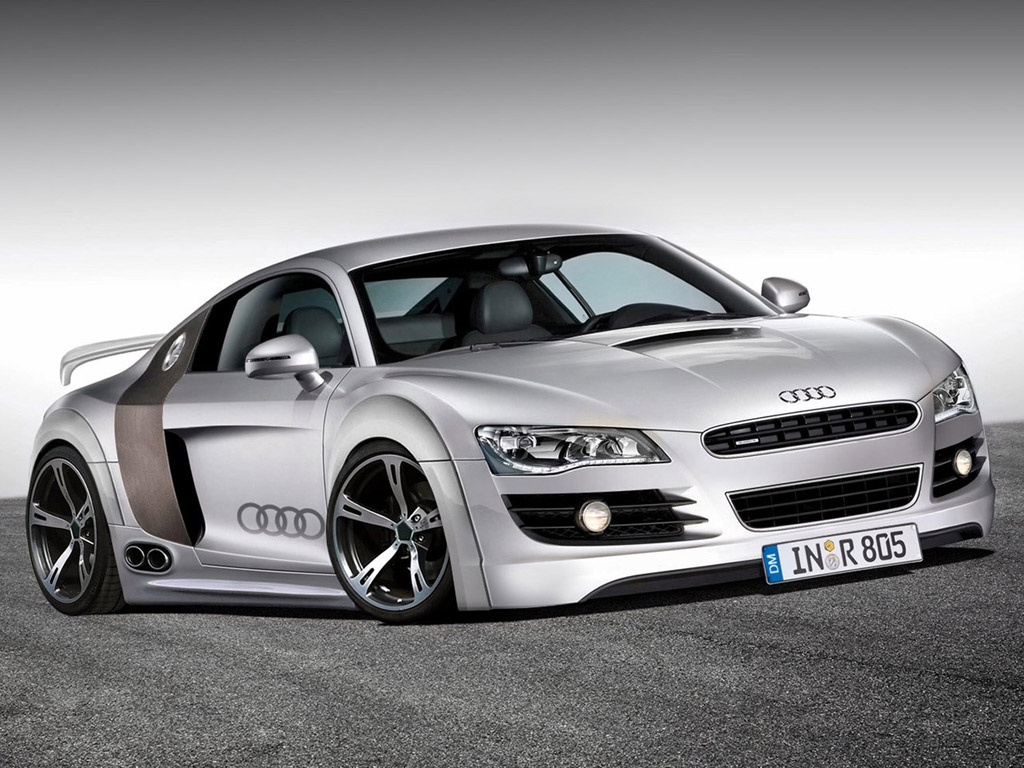
\includegraphics[scale = 0.08]{./images/car}}
%	\hspace{0.5em}
%	\fbox{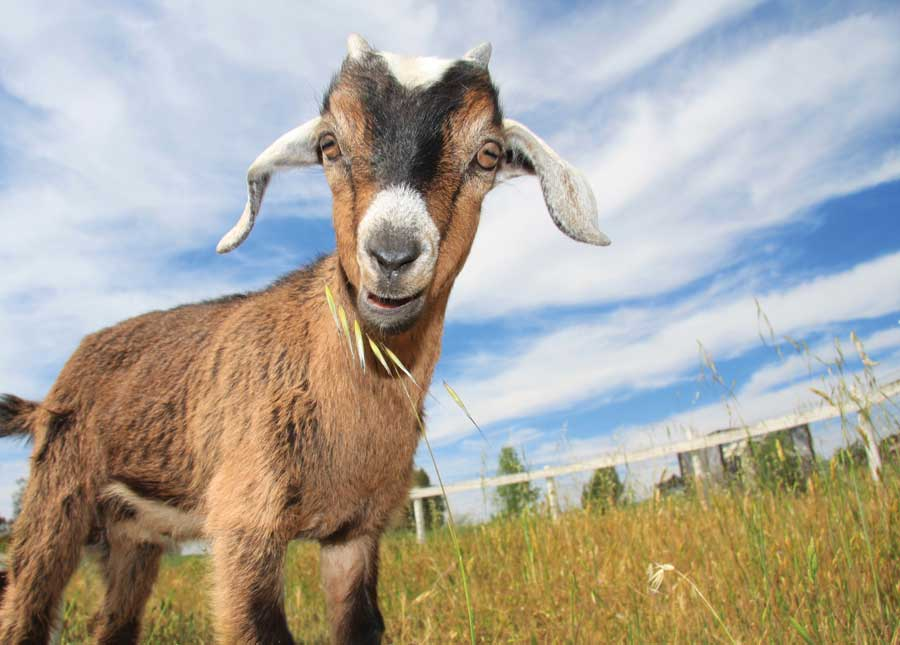
\includegraphics[scale = 0.095]{./images/goat}}
%	\hspace{0.5em}
%	\fbox{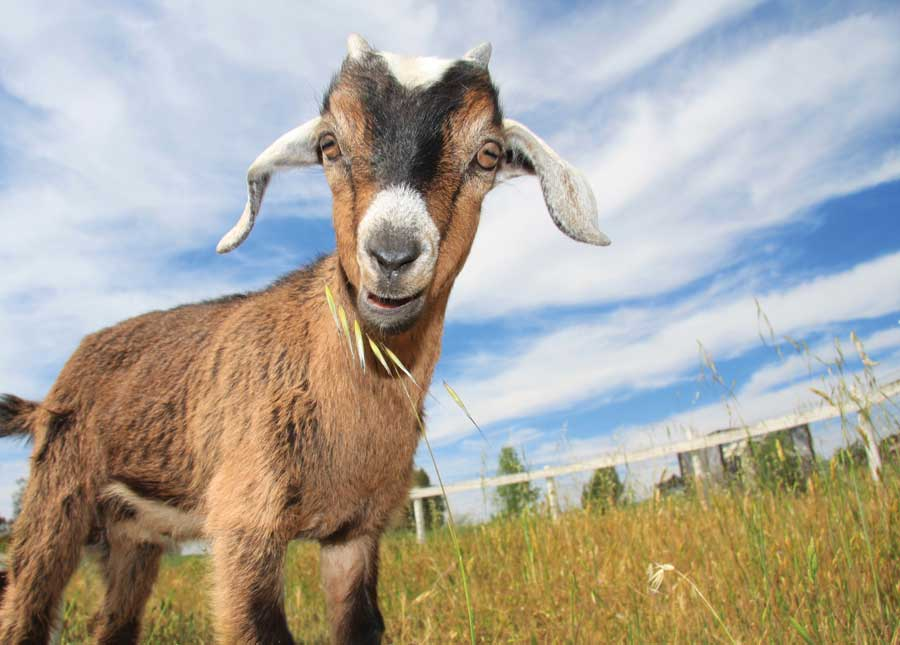
\includegraphics[scale = 0.095]{./images/goat}}
%\end{figure}
%\end{frame}
%%%%%%%%%%%%%%%%%%%%%%%%%%%%%%%%%%%%%%%%%
%
%
%\begin{frame}
%\frametitle{What is the probability that you win if you switch? \hfill 
\includegraphics[scale = 0.05]{./images/clicker}}
%\begin{figure}
%\centering
%	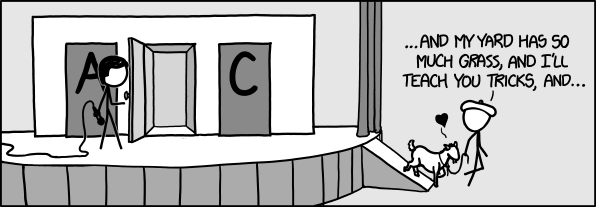
\includegraphics[scale = 0.55]{./images/monty_hall}
%\end{figure}
%\end{frame}
%
%%%%%%%%%%%%%%%%%%%%%%%%%%%%%%%%%%%%%%%%%%
%\begin{frame}
%
%\Huge Key Point -- Monte doesn't choose a door randomly: he \emph{always} shows you a goat.
%
%\end{frame}
%%%%%%%%%%%%%%%%%%%%%%%%%%%%%%%%%%%%%%%%%
%
%
%\begin{frame}
%\frametitle{Without loss of generality, suppose you chose door \#1}
%\begin{figure}[htbp]
%\begin{center}
%\small
%\synttree[Choose Door 1
%			[\emph{Car Behind Door 1}
%				[Switch	[\textbf{Lose}]	]	[Don't Switch	[\textbf{Win}]	]
%			]
%						[\emph{Car Behind Door 2}
%				[Switch	[\textbf{Win}]	]	[Don't Switch	[\textbf{Lose}]	]
%			]
%						[\emph{Car Behind Door 3}
%				[Switch	[\textbf{Win}]	]	[Don't Switch	[\textbf{Lose}]	]
%			]
%]
%\end{center}
%\end{figure}
%\end{frame}
%
%%%%%%%%%%%%%%%%%%%%%%%%%%%%%%%%%%%%%%%%%

\begin{frame}
  \begin{center}
  \Huge Random Variables
  \end{center}
\end{frame}
%%%%%%%%%%%%%%%%%%%%%%%%%%%%%%%%%%%%%%%%
%Some macros for diagrams of random variables
\def\RVraw{(-2.5,0) circle [radius=1.7]
	(-2.5,0) circle [radius=1.7]
	(2.5,0) circle [radius=1.7]
	node [above left] at (-3.75,1.25) {$S$}
	node [above right] at (3.75,1.25) {$\mathbb{R}$}
	%node [above] at (0,2) {$X\colon S \mapsto \mathbb{R}$}
}
%%%%%%%%%%%%%%%%%%%%%%%%%%%%%%%%%%%%%%%%
\begin{frame}
  \frametitle{Random Variables}
  \begin{quote}
    A random variable is neither random nor a variable.
  \end{quote}
\begin{block}{Random Variable (RV): $X$}
  A \emph{fixed} function that assigns a \emph{number} to each basic outcome of a random experimnet.
\end{block}
 
\begin{block}{Realization: $x$}
A particular numeric value that an RV could take on. We write $\{X = x\}$ to refer to the \emph{event} that the RV $X$ took on the value $x$.  
\end{block}
 
\begin{block}{Support Set (aka Support)}
The set of all possible realizations of a RV.
\end{block}
 
\end{frame}
%%%%%%%%%%%%%%%%%%%%%%%%%%%%%%%%%%%%%%%%
\begin{frame}
  \frametitle{Random Variables (continued)}
\begin{block}{Notation}
Capital latin letters for RVs, e.g.\ $X,Y,Z$, and the corresponsing lowercase letters for their realizations, e.g.\ $x,y,z$.
\end{block}

\begin{block}{Intuition}
  You can think of an RV as a machine that spits out random numbers: although the machine is deterministic, its inputs, the outcomes of a random experiment, are not.
\end{block}
\end{frame}
%%%%%%%%%%%%%%%%%%%%%%%%%%%%%%%%%%%%%%%%%
\begin{frame}
\frametitle{Example: Coin Flip Random Variable}

\begin{figure}
\centering
\begin{tikzpicture}
\draw \RVraw;
\draw [->] (-2.5,0.75) node [below]{Tails} to [out=35,in=145] (2.5,0.75) node [below]{$0$};
\draw [->] (-2.5,-0.75) node [above]{Heads} to [out=315,in=225] (2.5,-0.75) node [above]{$1$};
\end{tikzpicture}
\caption{This random variable assigns numeric values to the random experiment of flipping a fair coin once: Heads is assigned 1 and Tails 0.}
\end{figure}
\end{frame}
%%%%%%%%%%%%%%%%%%%%%%%%%%%%%%%%%%%%%%%%%%
\begin{frame}
  \frametitle{Which of these is a realization of the Coin Flip RV?\hfill
\includegraphics[scale = 0.05]{./images/clicker}}
  \begin{enumerate}[(a)]
    \item Tails
    \item 2
    \item 0 
    \item Heads
    \item 1/2
  \end{enumerate}
\end{frame}
%%%%%%%%%%%%%%%%%%%%%%%%%%%%%%%%%%%%%%%%%%
\begin{frame}
  \frametitle{What is the support set of the Coin Flip RV?\hfill
\includegraphics[scale = 0.05]{./images/clicker}}
  \begin{enumerate}[(a)]
    \item $\left\{ \mbox{Heads}, \mbox{Tails} \right\}$ 
    \item 1/2 
    \item 0 
    \item $\left\{ 0,1 \right\}$
    \item 1
  \end{enumerate}
\end{frame}
%%%%%%%%%%%%%%%%%%%%%%%%%%%%%%%%%%%%%%%%%%
\begin{frame}
  \frametitle{Let $X$ denote the Coin Flip RV \hfill
\includegraphics[scale = 0.05]{./images/clicker}}
  What is $P\left( X=1 \right)$?

  \vspace{1em}

  \begin{enumerate}[(a)]
    \item 0 
    \item 1  
    \item 1/2 
    \item Not enough information to determine
  \end{enumerate}
\end{frame}
%%%%%%%%%%%%%%%%%%%%%%%%%%%%%%%%%%%%%%%%%%
\begin{frame}
  \frametitle{Two Kinds of RVs: Discrete and Continuous}
  \begin{description}
    \item[Discrete] support set is discrete, e.g.\ $\left\{ 0,1,2 \right\}$,  $\left\{ \hdots, -2, -1, 0, 1, 2,\hdots \right\}$
    \item[Continuous] support set is continuous, e.g.\ $[-1,1]$, $\mathbb{R}$.
  \end{description}

  \vspace{1em}

  \alert{Start with the discrete case since it's easier, but most of the ideas we learn will carry over to the continuous case.}
\end{frame}
%%%%%%%%%%%%%%%%%%%%%%%%%%%%%%%%%%%%%%%%%%
\begin{frame}

\centering \Huge Discrete Random Variables I

\end{frame}
%%%%%%%%%%%%%%%%%%%%%%%%%%%%%%%%%%%%%%%%
\begin{frame}
\frametitle{Probability Mass Function (pmf)}
 A function that gives $P(X=x)$ for any realization $x$ in the support set of a discrete RV $X$. We use the following notation for the pmf:
 $$p(x) = P(X =x)$$

 

\begin{alertblock}{Plug in a realization $x$, get out a probability  $p(x)$.}\end{alertblock}

 


\end{frame}
%%%%%%%%%%%%%%%%%%%%%%%%%%%%%%%%%%%%%%%%
\begin{frame}
\frametitle{Probability Mass Function for Coin Flip RV}

\begin{columns}
\column{0.25\textwidth}
$$X = \left\{ \begin{array}{l}  0, \mbox{Tails}\\ 1, \mbox{Heads}\end{array} \right.$$

\begin{eqnarray*}
	p(0) &=& 1/2\\
	p(1) &=& 1/2
\end{eqnarray*}


\column{0.75\textwidth}
\begin{figure}
\centering
\begin{tikzpicture}[scale = 1.5]
\draw [<->] (0,2) node [above]{$p(x)$} -- (0,0) -- (3,0) node [right]{$x$};
\draw [blue, thick] (0.75,0) node [black, below]{0} -- (0.75,1.5);
\draw [blue, thick] (2.25,0) node [black, below]{1} -- (2.25,1.5);
\draw [dashed, gray] (0, 1.5) node [black, left]{$1/2$} -- (3,1.5);
\draw [fill=blue] (2.25,1.51) circle [radius = 0.05];
\draw [fill=blue] (0.75,1.51) circle [radius = 0.05];
\end{tikzpicture}
\caption{Plot of pmf for Coin Flip Random Variable}
\end{figure}
\end{columns}


\end{frame}
%%%%%%%%%%%%%%%%%%%%%%%%%%%%%%%%%%%%%%%%


\begin{frame}
\frametitle{Important Note about Support Sets}
Whenever you write down the pmf of a RV, it is \alert{crucial} to also write down its Support Set. Recall that this is the set of \alert{\emph{all possible realizations for a RV}}. Outside of the support set, all probabilities are zero. In other words, the pmf is \alert{only defined} on the support.

\end{frame}
%%%%%%%%%%%%%%%%%%%%%%%%%%%%%%%%%%%%%%%%
\begin{frame}
\frametitle{Properties of Probability Mass Functions}

If $p(x)$ is the pmf of a random variable $X$, then
\begin{enumerate}[(i)]
	\item $0\leq p(x) \leq 1$ for all $x$ \vspace{1em}
	\item $\displaystyle \sum_{\mbox{all } x} p(x) = 1$
\end{enumerate}

\vspace{0.75em}
where ``all $x$'' is shorthand for ``all $x$ in the support of $X$.''
%%%%%%%%%%%%%%%%%%%%%%%%%%%%%%%%%%%%%%%%

\end{frame}

\end{document}
